
In this section, we present the high-level architecture of the CONFINE framework. We consider the main functionalities of each component, avoiding details on the employed technologies discussed in the next sections. %After introducing the architecture, we focus on the \emph{Secure Miner}, a core component of our contribution.
\begin{figure}[t]
	\centering
	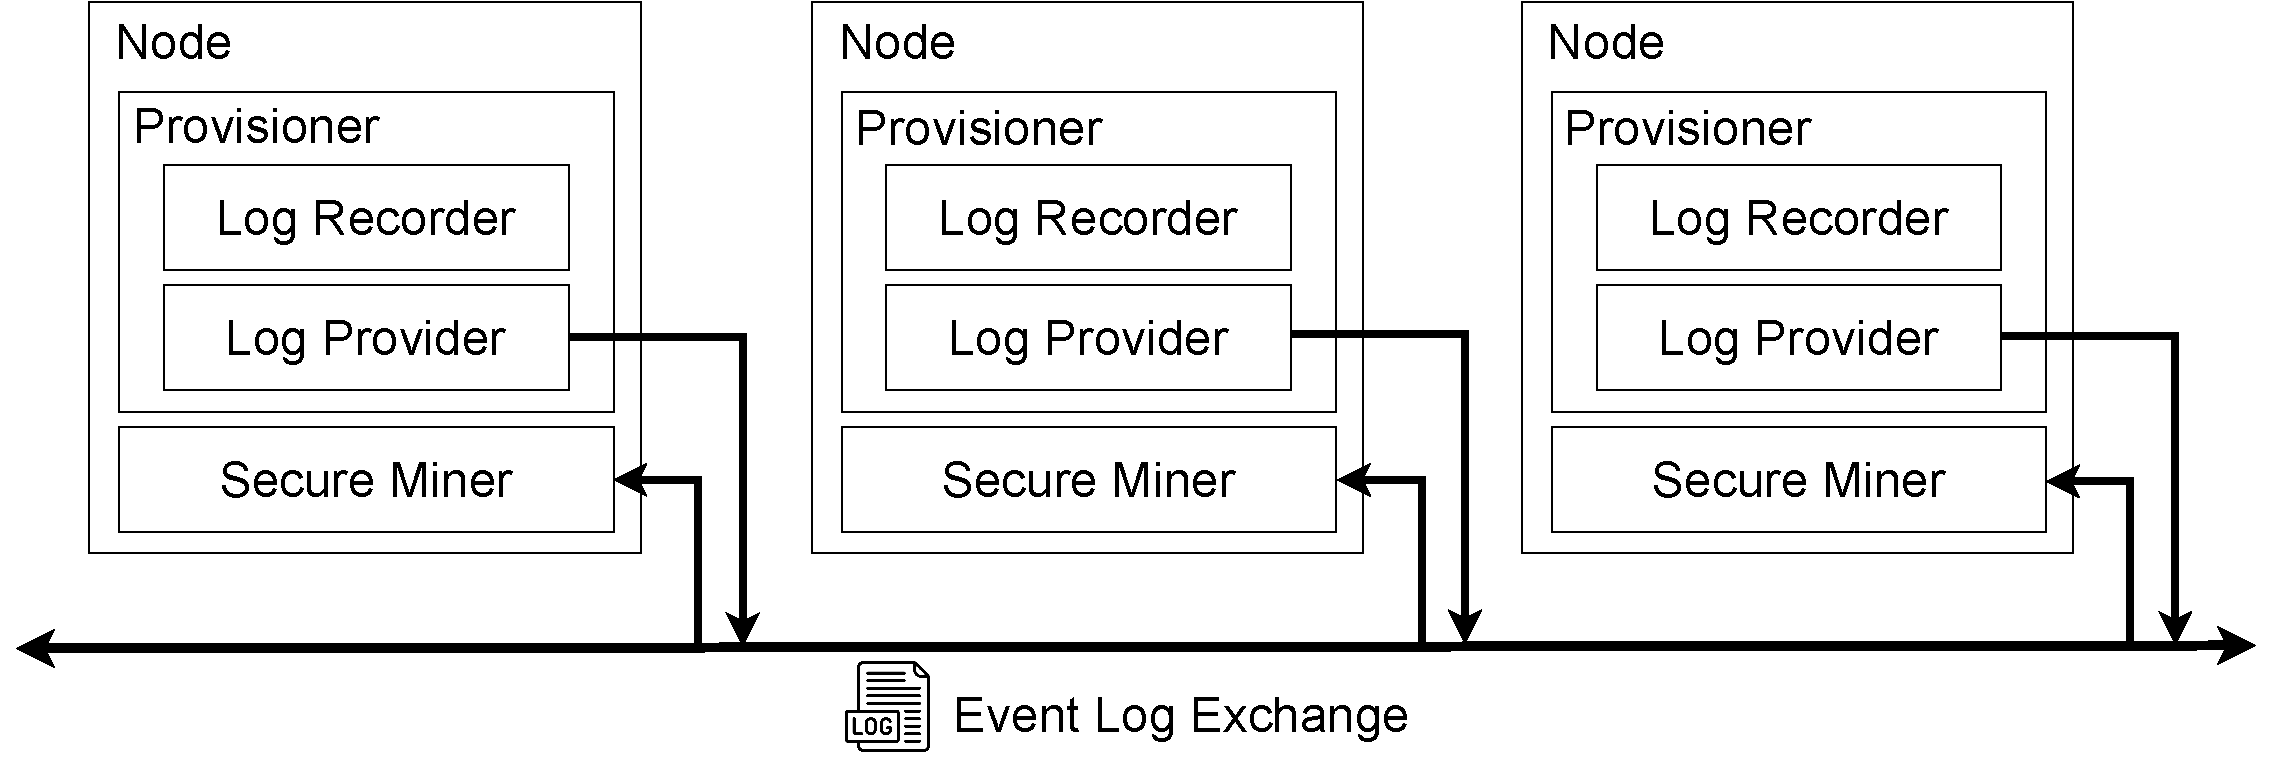
\includegraphics[width=0.79\linewidth]{content/figures/architecturediagram.pdf}
	\caption{The CONFINE high-level architecture}
	\label{fig:architecture_diagram}
\end{figure}

\begin{wrapfigure}[9]{r}{0.4\textwidth}
	\vspace{-2em}
	\centering
	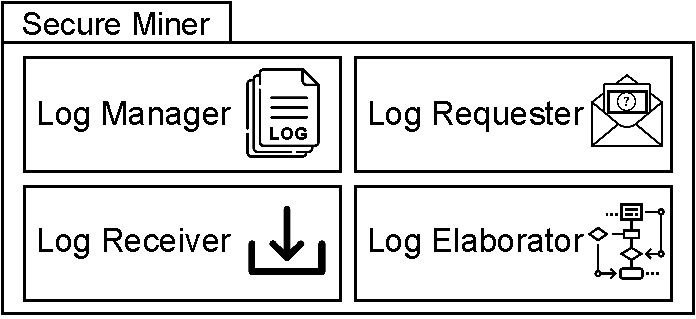
\includegraphics[width=1\textwidth]{content/figures/secureminersad.pdf}
	\caption[Secure Miner sub-components]{Sub-components of the \\Secure Miner}
	\label{fig:trusted_miner}
	\vspace{-6pt}
\end{wrapfigure} 

\noindent\textbf{The CONFINE architecture at large.}
Our architecture involves different information systems running on multiple machines. An organization can take at least one of the following roles: 
\begin{inparadesc}
\item[provisioning] if it delivers local event logs to be collaboratively mined;
\item[mining] if it applies process mining algorithms using event logs retrieved from provisioners.
\end{inparadesc}
In \cref{fig:architecture_diagram}, we propose the high-level schematization of the CONFINE framework.
In our solution, every organization hosts one or more nodes hosting components (the names of which will henceforth be formatted with a \Compo{teletype} font). Depending on the played role, nodes come endowed with a \Compo{Provisioner} or a \Compo{Secure Miner} component, or both. The \Compo{Provisioner} component consists of the following two main sub-components. The \begin{inparadesc}
\item[\Compo{Log Recorder}] registers the events taking place in the organizations' systems. The
\item[\Compo{Log Provider}] delivers on-demand data to mining players.
\end{inparadesc}
The \Actor{Hospital} and all other parties in our example record Alice and Bob's cases using the \Compo{Log Recorder}. The \Compo{Log Recorder} is queried by the \Compo{Log Provider} for event logs to be made available for mining. The latter controls access to local event logs by authenticating data requests by miners and rejecting those that come from unauthorized parties.
In our motivating scenario, the \Actor{Specialized clinic}, the \Actor{Pharmaceutical company}, and the \Actor{Hospital} leverage \Compo{Log Provider}s to authenticate the miner party before sending their logs.  The \Compo{Secure Miner} component
% \Compo{Log Provider}s reject demands from unauthorized parties and only permit \texttt{Secure Miners} to use the data. 
% The \Compo{Secure Miner} 
shelters external event logs inside a protected environment to preserve data confidentiality and integrity.
Notice that \Compo{Log Provider}s accept requests issued solely by \Compo{Secure Miner}s. 
Next, we provide an in-depth focus on the latter.
% We provide an in-depth focus on this key component in the following.


\noindent\textbf{The Secure Miner.}
The primary objective of the \Compo{Secure Miner} is to allow miners to securely execute process mining algorithms using event logs retrieved from provisioners such as the \Actor{Specialized clinic}, \Actor{Pharmaceutical company}, and the \Actor{Hospital} in our example. \Compo{Secure Miner}s are isolated components that guarantee data inalterability and confidentiality. In \cref{fig:trusted_miner}, we show a schematization of the \Compo{Secure Miner}, which consists of four sub-components:
\begin{inparaenum}[\itshape(i)\upshape]
    \item \Compo{Log Requester};
    \item \Compo{Log Receiver};
    \item \Compo{Log Manager}; 
    \item \Compo{Log Elaborator}.
\end{inparaenum}
%Event logs belonging to provisioners are locked in the \Compo{Secure Miner}.
%We handle  data via the 
The \Compo{Log Requester} and the \Compo{Log Receiver} are the sub-components that we employ during the event log retrieval. \Compo{Log Requester}s send authenticable data requests to the \Compo{Log Provider}s. The \Compo{Log Receiver} collects event logs sent by \texttt{Log Providers} and entrusts them to the \Compo{Log Manager}, securing them from accesses that are external to the \Compo{Secure Miner}.
Miners of our motivating scenario, such as the \Actor{University} and the \Actor{National Institute of Statistics}, employ these three components to retrieve and store Alice and Bob's data. The \Compo{Log Elaborator} merges the event data locked in the \Compo{Secure Miner} to have a global view of the inter-organizational process comprehensive of activities executed by each involved party. Thereupon, it executes process mining algorithms in a protected environment, inaccessible from the outside computation environment.
In our motivating scenario, the \Compo{Log Elaborator} combines the traces associated with the cases of Alice (i.e., $T^H_{312}$, $T^S_{312}$, and $T^C_{312}$) and Bob (i.e, $T^H_{711}$, $T^S_{711}$, and $T^C_{711}$), generates the chronologically sorted traces $T_{312}$ and $T_{711}$, and feeds them into the mining algorithms (see the bottom-right quadrant of \cref{tab:trace}).



